\section{Testy wydajnościowe}

\subsection{Zależność czasowa od liczby pikseli}


\begin{figure}[!ht]
\advance\leftskip-2cm
\begin{subfigure}{.5\textwidth}
    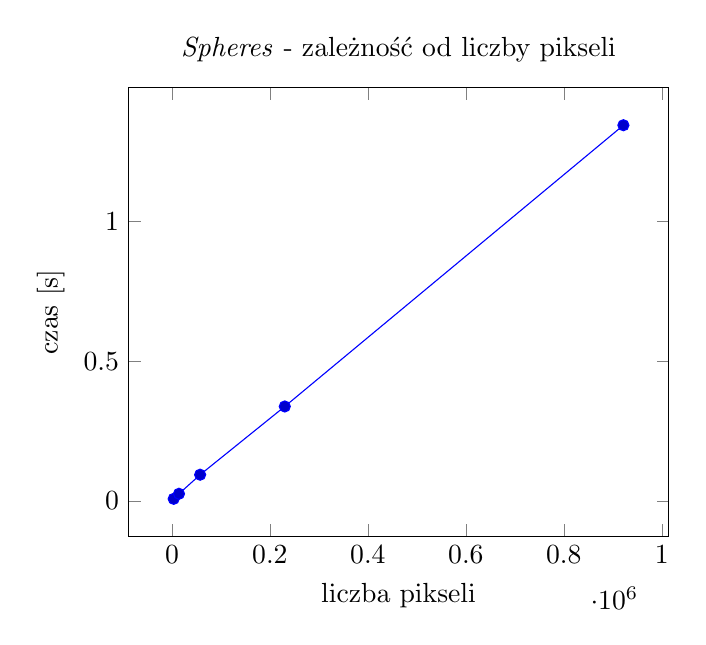
\begin{tikzpicture}
	  \begin{axis}[
	    title=\emph{Spheres} - zależność od liczby pikseli,
	    xlabel=liczba pikseli,
	    ylabel=czas \lbrack s\rbrack,]
	    \addplot coordinates {(3600,0.00764382) (14400,0.0257124) (57600,0.093867) (230400,0.337877) (921600,1.3434)};
	    % if you want the plot to be RED, instead write: \addplot [red,mark=*] coordinates ...
	  \end{axis}
	\end{tikzpicture}
\end{subfigure}
\hspace{2cm}
\begin{subfigure}{.5\textwidth}
		\begin{longtable}{|c|c|c|} \hline
	    liczba pikseli & fps & spf \\ \hline
	    3600 & 130,825 & 0,00764382 \\ 
	    14400 &	38,8918 & 0,0257124 \\
		57600 & 10,6533 & 0,093867 \\
		230400 & 2,95966 & 0,337877 \\
		921600 & 0,74438 & 1,3434 \\
		\hline
		\end{longtable}
\end{subfigure}
\end{figure}

\begin{figure}[!ht]
\advance\leftskip-2cm
\begin{subfigure}{.5\textwidth}
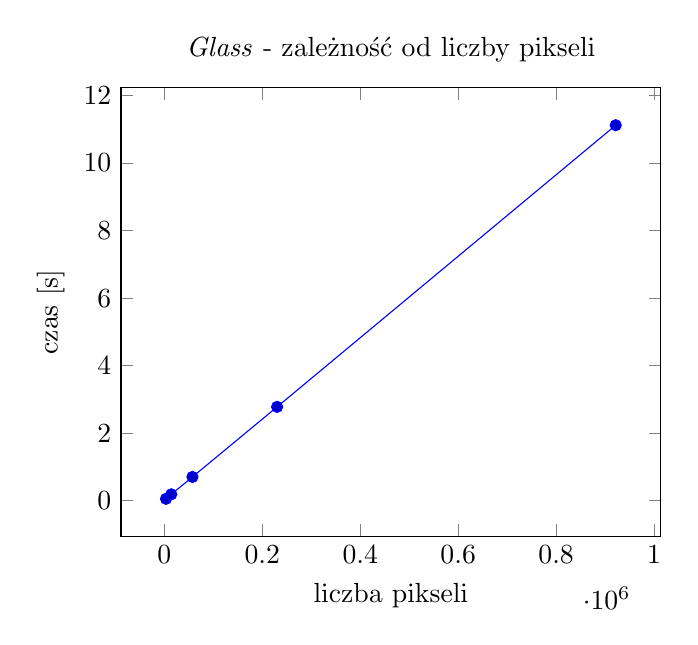
\begin{tikzpicture}
  \begin{axis}[
    title=\emph{Glass} - zależność od liczby pikseli,
    xlabel=liczba pikseli,
    ylabel=czas \lbrack s\rbrack,]
    \addplot coordinates {(3600,0.0567306) (14400,0.191007) (57600,0.705118) (230400,2.77945) (921600,11.1171)};
    % if you want the plot to be RED, instead write: \addplot [red,mark=*] coordinates ...
  \end{axis}
\end{tikzpicture}
\end{subfigure}
\hspace{2cm}
\begin{subfigure}{.5\textwidth}
		\begin{longtable}{|c|c|c|} \hline
	    liczba pikseli & fps & spf \\ \hline
	    3600 & 130,825 & 0,00764382 \\ 
	    14400 &	38,8918 & 0,0257124 \\
		57600 & 10,6533 & 0,093867 \\
		230400 & 2,95966 & 0,337877 \\
		921600 & 0,74438 & 1,3434 \\
		\hline
		\end{longtable}
\end{subfigure}
\end{figure}

\begin{figure}[!ht]
\advance\leftskip-2cm
\begin{subfigure}{.5\textwidth}
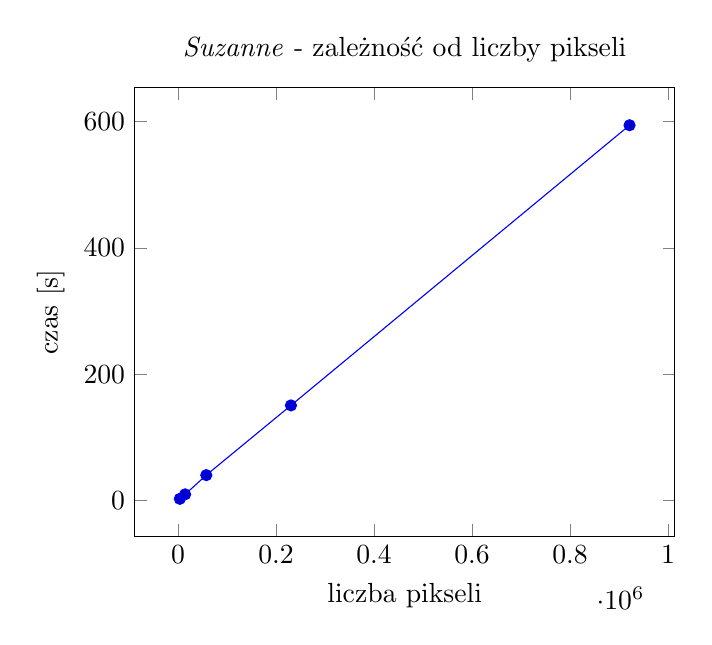
\begin{tikzpicture}
  \begin{axis}[
    title=\emph{Suzanne} - zależność od liczby pikseli,
    xlabel=liczba pikseli,
    ylabel=czas \lbrack s\rbrack,]
    \addplot coordinates {(3600,2.67767) (14400,9.73898) (57600,40.1629) (230400,150.539) (921600,594.091)};
    % if you want the plot to be RED, instead write: \addplot [red,mark=*] coordinates ...
  \end{axis}
\end{tikzpicture}
\end{subfigure}
\hspace{2cm}
\begin{subfigure}{.5\textwidth}
		\begin{longtable}{|c|c|c|} \hline
	    liczba pikseli & fps & spf \\ \hline
	    3600 & 130,825 & 0,00764382 \\ 
	    14400 &	38,8918 & 0,0257124 \\
		57600 & 10,6533 & 0,093867 \\
		230400 & 2,95966 & 0,337877 \\
		921600 & 0,74438 & 1,3434 \\
		\hline
		\end{longtable}
\end{subfigure}
\end{figure}


\begin{figure}[!ht]
\advance\leftskip-2cm
\begin{subfigure}{.5\textwidth}
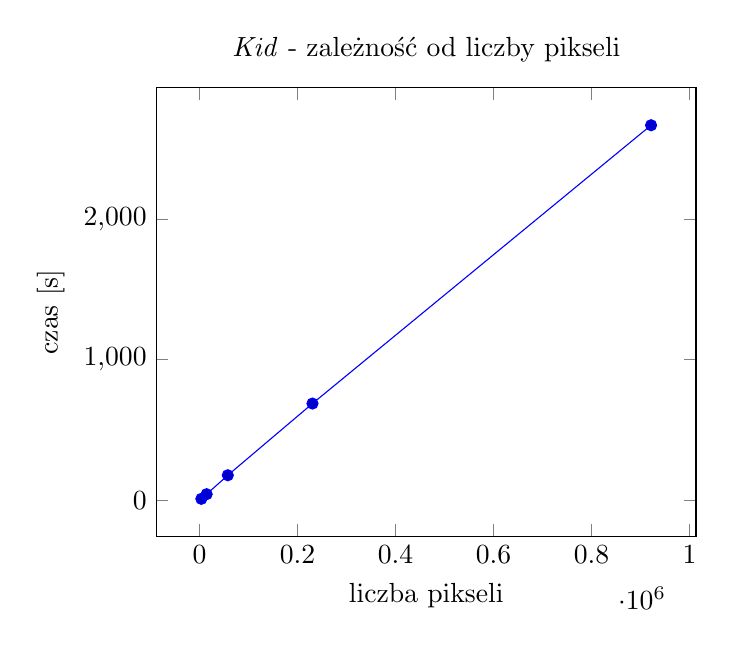
\begin{tikzpicture}
  \begin{axis}[
    title=\emph{Kid} - zależność od liczby pikseli,
    xlabel=liczba pikseli,
    ylabel=czas \lbrack s\rbrack,]
    \addplot coordinates {(3600,11.0737) (14400,44.1641) (57600,178.688) (230400,688.478) (921600,2666.95)};
    % if you want the plot to be RED, instead write: \addplot [red,mark=*] coordinates ...
  \end{axis}
\end{tikzpicture}
\end{subfigure}
\hspace{2cm}
\begin{subfigure}{.5\textwidth}
		\begin{longtable}{|c|c|c|} \hline
	    liczba pikseli & fps & spf \\ \hline
	    3600 & 130,825 & 0,00764382 \\ 
	    14400 &	38,8918 & 0,0257124 \\
		57600 & 10,6533 & 0,093867 \\
		230400 & 2,95966 & 0,337877 \\
		921600 & 0,74438 & 1,3434 \\
		\hline
		\end{longtable}
\end{subfigure}
\end{figure}

\subsection{Zależność czasowa od głębokości drzewa}

\begin{figure}[!ht]
\advance\leftskip-2cm
\begin{subfigure}{.5\textwidth}
\begin{tikzpicture}
  \begin{axis}[
    title=\emph{Spheres} - zależność od głębokości drzewa,
    xlabel=głębokość,
    ylabel=czas \lbrack s\rbrack,]
    \addplot coordinates {(1,0.142384) (2,0.240045) (4,0.444783) (8,0.852983) (16,1.6478)};
    % if you want the plot to be RED, instead write: \addplot [red,mark=*] coordinates ...
  \end{axis}
\end{tikzpicture}
\end{subfigure}
\hspace{2cm}
\begin{subfigure}{.5\textwidth}
		\begin{longtable}{|c|c|c|} \hline
	    liczba pikseli & fps & spf \\ \hline
	    3600 & 130,825 & 0,00764382 \\ 
	    14400 &	38,8918 & 0,0257124 \\
		57600 & 10,6533 & 0,093867 \\
		230400 & 2,95966 & 0,337877 \\
		921600 & 0,74438 & 1,3434 \\
		\hline
		\end{longtable}
\end{subfigure}
\end{figure}


\begin{figure}[!ht]
\advance\leftskip-2cm
\begin{subfigure}{.5\textwidth}
\begin{tikzpicture}
  \begin{axis}[
    title=\emph{Glass} - zależność od głębokości drzewa,
    xlabel=głębokość,
    ylabel=czas \lbrack s\rbrack,]
    \addplot coordinates {(1,2.16837) (2,2.69988) (4,2.84109) (8,2.86541) (16,2.84629)};
    % if you want the plot to be RED, instead write: \addplot [red,mark=*] coordinates ...
  \end{axis}
\end{tikzpicture}
\end{subfigure}
\hspace{2cm}
\begin{subfigure}{.5\textwidth}
		\begin{longtable}{|c|c|c|} \hline
	    liczba pikseli & fps & spf \\ \hline
	    3600 & 130,825 & 0,00764382 \\ 
	    14400 &	38,8918 & 0,0257124 \\
		57600 & 10,6533 & 0,093867 \\
		230400 & 2,95966 & 0,337877 \\
		921600 & 0,74438 & 1,3434 \\
		\hline
		\end{longtable}
\end{subfigure}
\end{figure}

\begin{figure}[!ht]
\advance\leftskip-2cm
\begin{subfigure}{.5\textwidth}
\begin{tikzpicture}
  \begin{axis}[
    title=\emph{Suzanne} - zależność od głębokości drzewa,
    xlabel=głębokość,
    ylabel=czas \lbrack s\rbrack,]
    \addplot coordinates {(1,129.559) (2,150.077) (4,149.244) (8,151.812) (16,153.429)};
    % if you want the plot to be RED, instead write: \addplot [red,mark=*] coordinates ...
  \end{axis}
\end{tikzpicture}
\end{subfigure}
\hspace{2cm}
\begin{subfigure}{.5\textwidth}
		\begin{longtable}{|c|c|c|} \hline
	    liczba pikseli & fps & spf \\ \hline
	    3600 & 130,825 & 0,00764382 \\ 
	    14400 &	38,8918 & 0,0257124 \\
		57600 & 10,6533 & 0,093867 \\
		230400 & 2,95966 & 0,337877 \\
		921600 & 0,74438 & 1,3434 \\
		\hline
		\end{longtable}
\end{subfigure}
\end{figure}

\begin{figure}[!ht]
\advance\leftskip-2cm
\begin{subfigure}{.5\textwidth}
\begin{tikzpicture}
  \begin{axis}[
    title=\emph{Kid} - zależność od głębokości drzewa,
    xlabel=głębokość,
    ylabel=czas \lbrack s\rbrack,]
    \addplot coordinates {(1,230.193) (2,432.88) (4,843.196) (8,1303.88) (16,1718.51)};
    % if you want the plot to be RED, instead write: \addplot [red,mark=*] coordinates ...
  \end{axis}
\end{tikzpicture}
\end{subfigure}
\hspace{2cm}
\begin{subfigure}{.5\textwidth}
		\begin{longtable}{|c|c|c|} \hline
	    liczba pikseli & fps & spf \\ \hline
	    3600 & 130,825 & 0,00764382 \\ 
	    14400 &	38,8918 & 0,0257124 \\
		57600 & 10,6533 & 0,093867 \\
		230400 & 2,95966 & 0,337877 \\
		921600 & 0,74438 & 1,3434 \\
		\hline
		\end{longtable}
\end{subfigure}
\end{figure}




\subsection{Zależność czasowa od światła}

\begin{figure}[!ht]
\advance\leftskip-2cm
\begin{subfigure}{.5\textwidth}
\begin{tikzpicture}
  \begin{axis}[
    title=\emph{Spheres} - zależność od światła,
    xlabel=głębokość,
    ylabel=czas \lbrack s\rbrack,]
    \addplot coordinates {(1,0.251023) (2,0.329837) (4,0.482877) (8,0.786847) (16,1.48653)};
    \addplot coordinates {(1,0.284545) (2,0.318328) (4,0.395992) (8,0.561186) (16,0.561186)};
    % if you want the plot to be RED, instead write: \addplot [red,mark=*] coordinates ...
  \end{axis}
\end{tikzpicture}
\end{subfigure}
\hspace{2cm}
\begin{subfigure}{.5\textwidth}
		\begin{longtable}{|c|c|c|} \hline
	    liczba pikseli & fps & spf \\ \hline
	    3600 & 130,825 & 0,00764382 \\ 
	    14400 &	38,8918 & 0,0257124 \\
		57600 & 10,6533 & 0,093867 \\
		230400 & 2,95966 & 0,337877 \\
		921600 & 0,74438 & 1,3434 \\
		\hline
		\end{longtable}
\end{subfigure}
\end{figure}

\begin{figure}[!ht]
\advance\leftskip-2cm
\begin{subfigure}{.5\textwidth}
\begin{tikzpicture}
  \begin{axis}[
    title=\emph{Glass} - zależność od światła,
    xlabel=głębokość,
    ylabel=czas \lbrack s\rbrack,]
    \addplot coordinates {(1,2.88157) (2,2.76963) (4,2.78286) (8,2.81478) (16,2.88768)};
    \addplot coordinates {(1,3.27412) (2,3.76403) (4,5.1113) (8,7.44586) (16,10.9446)};
    % if you want the plot to be RED, instead write: \addplot [red,mark=*] coordinates ...
  \end{axis}
\end{tikzpicture}
\end{subfigure}
\hspace{2cm}
\begin{subfigure}{.5\textwidth}
		\begin{longtable}{|c|c|c|} \hline
	    liczba pikseli & fps & spf \\ \hline
	    3600 & 130,825 & 0,00764382 \\ 
	    14400 &	38,8918 & 0,0257124 \\
		57600 & 10,6533 & 0,093867 \\
		230400 & 2,95966 & 0,337877 \\
		921600 & 0,74438 & 1,3434 \\
		\hline
		\end{longtable}
\end{subfigure}
\end{figure}

\begin{figure}[!ht]
\advance\leftskip-2cm
\begin{subfigure}{.5\textwidth}
\begin{tikzpicture}
  \begin{axis}[
    title=\emph{Suzanne} - zależność od światła,
    xlabel=głębokość,
    ylabel=czas \lbrack s\rbrack,]
    \addplot coordinates {(1,151.408) (2,155.419) (4,162.98) (8,154.59) (16,173.54)};
    \addplot coordinates {(1,146.452) (2,164.65) (4,168.411) (8,201.321) (16,248.212)};
    % if you want the plot to be RED, instead write: \addplot [red,mark=*] coordinates ...
  \end{axis}
\end{tikzpicture}
\end{subfigure}
\hspace{2cm}
\begin{subfigure}{.5\textwidth}
		\begin{longtable}{|c|c|c|} \hline
	    liczba pikseli & fps & spf \\ \hline
	    3600 & 130,825 & 0,00764382 \\ 
	    14400 &	38,8918 & 0,0257124 \\
		57600 & 10,6533 & 0,093867 \\
		230400 & 2,95966 & 0,337877 \\
		921600 & 0,74438 & 1,3434 \\
		\hline
		\end{longtable}
\end{subfigure}
\end{figure}


\begin{figure}[!ht]
\advance\leftskip-2cm
\begin{subfigure}{.5\textwidth}
\begin{tikzpicture}
  \begin{axis}[
    title=\emph{Kid} - zależność od światła,
    xlabel=głębokość,
    ylabel=czas \lbrack s\rbrack,]
    \addplot coordinates {(1,705.337) (2,716.45) (4,714.296) (8,848.262) (16,853.408)};
    \addplot coordinates {(1,1040.56) (2,1435.52) (4,2330.47) (8,3904.24) (16,6871.04)};
    % if you want the plot to be RED, instead write: \addplot [red,mark=*] coordinates ...
  \end{axis}
\end{tikzpicture}
\end{subfigure}
\hspace{2cm}
\begin{subfigure}{.5\textwidth}
		\begin{longtable}{|c|c|c|} \hline
	    liczba pikseli & fps & spf \\ \hline
	    3600 & 130,825 & 0,00764382 \\ 
	    14400 &	38,8918 & 0,0257124 \\
		57600 & 10,6533 & 0,093867 \\
		230400 & 2,95966 & 0,337877 \\
		921600 & 0,74438 & 1,3434 \\
		\hline
		\end{longtable}
\end{subfigure}
\end{figure}


\subsection{Zależność czasowa w zależności od zrównoleglenia}

%%%%%%%%%%%%%%%%%%%%%%%%%%%%%%%%%%%%%%%%%%%%%%%%%%%
\begin{figure}[!ht][ht!]
\advance\leftskip-2cm
	\begin{subfigure}{.5\textwidth}
	\begin{tikzpicture}
	  \begin{axis}[
	    title=\emph{Spheres} - zależność od zrównoleglenia (320x180),
	    xlabel=głębokość,
	    ylabel=czas \lbrack s\rbrack,]
	    \addplot coordinates {(16,0.0574393) (36,0.0716171) (64,0.0925856) (100,0.192079) (144,0.208692)};
	    \addplot coordinates {(16,0.0383637) (36,0.0636916) (64,0.10683) (100,0.145227) (144,0.221282)};
	    \addplot coordinates {(16,0.0270853) (36,0.0619941) (64,0.0969651) (100,0.165164) (144,0.204808)};
	    % if you want the plot to be RED, instead write: \addplot [red,mark=*] coordinates ...
	  \end{axis}
	\end{tikzpicture}
	\end{subfigure}
	\hspace{2cm}
	\begin{subfigure}{.5\textwidth}
	\begin{tikzpicture}
	  \begin{axis}[
	    title=\emph{Spheres} - zależność od zrównoleglenia (640x360),
	    xlabel=głębokość,
	    ylabel=czas \lbrack s\rbrack,]
	    \addplot coordinates {(16,0.179093) (36,0.170406) (64,0.206508) (100,0.213478) (144,0.252288)};
	    \addplot coordinates {(16,0.0881486) (36,0.0854354) (64,0.103843) (100,0.145735) (144,0.218693)};
	    \addplot coordinates {(16,0.0619428) (36,0.063786) (64,0.0976417) (100,0.145701) (144,0.217703)};
	    % if you want the plot to be RED, instead write: \addplot [red,mark=*] coordinates ...
	  \end{axis}
	\end{tikzpicture}
	\end{subfigure}
\end{figure}
%%%%%%%%%%%%%%%%%%%%%%%%%%%%%%%%%%%%%%%%%%%%%%%%%%%%%%%%%%%%
%%%%
\begin{tabular}{|c|c|c|c|c|c|c|} \hline
	    \multirow{2}{*}{\backslashbox{chunks}{n}} & \multicolumn{2}{|c|}{5} & \multicolumn{2}{|c|}{10} & \multicolumn{2}{|c|}{15} \\ \cline{2-7}
	 	& spf & fps & spf & fps & spf & fps \\ \hline
	    16 & 130,825 & 0,00764382 & & & & \\ 
	    36 & 38,8918 & 0,0257124 & & & & \\
		64 & 10,6533 & 0,093867 & & & & \\
		100 & 2,95966 & 0,337877 & & & & \\
		144 & 0,74438 & 1,3434  & & & & \\ \hline
		max przysp. & & & & & & \\
		\hline
\end{tabular}
%%%%
%%%%%%%%%%%%%%%%%%%%%%%%%%%%%%%%%%%%%%%%%%%%%%%%%%%%%%%%%%%%%%%%
\begin{figure}[!ht]
\advance\leftskip-2cm
	\begin{subfigure}{.5\textwidth}
	\begin{tikzpicture}
	  \begin{axis}[
	    title=\emph{Glass} - zależność od zrównoleglenia (320x180),
	    xlabel=głębokość,
	    ylabel=czas \lbrack s\rbrack,]
	    \addplot coordinates {(16,0.313794) (36,0.308252) (64,0.327707) (100,0.376798) (144,0.411532)};
	    \addplot coordinates {(16,0.156765) (36,0.130717) (64,0.15545) (100,0.170898) (144,0.237513)};
	    \addplot coordinates {(16,0.156044) (36,0.106895) (64,0.110286) (100,0.174972) (144,0.229939)};
	    % if you want the plot to be RED, instead write: \addplot [red,mark=*] coordinates ...
	  \end{axis}
	\end{tikzpicture}	
	\end{subfigure}
	\hspace{2cm}
	\begin{subfigure}{.5\textwidth}
	\begin{tikzpicture}
	  \begin{axis}[
	    title=\emph{Glass} - zależność od zrównoleglenia (640x360),
	    xlabel=głębokość,
	    ylabel=czas \lbrack s\rbrack,]
	    \addplot coordinates {(16,1.09964) (36,1.05298) (64,1.03611) (100,1.02236) (144,1.05367)};
	    \addplot coordinates {(16,0.742264) (36,0.548189) (64,0.513832) (100,0.507293) (144,0.544521)};
	    \addplot coordinates {(16,0.479671) (36,0.407425) (64,0.311017) (100,0.322993) (144,0.344262)};
	    % if you want the plot to be RED, instead write: \addplot [red,mark=*] coordinates ...
	  \end{axis}
	\end{tikzpicture}
	\end{subfigure}
\end{figure}
%%%%%%%%%%%%%%%%%%%%%%%%%%%%%%%%%%%%%%%%%%%%%%%%%%%%%%%%%%%%%%%%%%%%
%
%
%%%%%%%%%%%%%%%%%%%%%%%%%%%%%%%%%%%%%%%%%%%%%%%%%%%%%%%%%%%%%%%%
\begin{figure}[!ht]
\advance\leftskip-2cm
	\begin{subfigure}{.5\textwidth}
	\begin{tikzpicture}
	  \begin{axis}[
	    title=\emph{Suzanne} - zależność od zrównoleglenia (320x180),
	    xlabel=głębokość,
	    ylabel=czas \lbrack s\rbrack,]
	    \addplot coordinates {(16,52.4239) (36,50.7791) (64,51.7074) (100,51.8617) (144,51.0035)};
	    \addplot coordinates {(16,18.8889) (36,17.8706) (64,18.3656) (100,18.1192) (144,17.5219)};
	    \addplot coordinates {(16,14.092) (36,9.19942) (64,9.82458) (100,9.43981) (144,9.47942)};
	    % if you want the plot to be RED, instead write: \addplot [red,mark=*] coordinates ...
	  \end{axis}
	\end{tikzpicture}
	\end{subfigure}
	\hspace{2cm}
	\begin{subfigure}{.5\textwidth}
	\begin{tikzpicture}
	  \begin{axis}[
	    title=\emph{Suzanne} - zależność od zrównoleglenia (640x360),
	    xlabel=głębokość,
	    ylabel=czas \lbrack s\rbrack,]
	    \addplot coordinates {(16,205.605) (36,206.972) (64,209.42) (100,217.794) (144,205.472)};
	    \addplot coordinates {(16,75.4728) (36,70.136) (64,71.2841) (100,70.7879) (144,71.007)};
	    \addplot coordinates {(16,52.8091) (36,37.398) (64,39.9895) (100,37.832) (144,37.0606)};
	    % if you want the plot to be RED, instead write: \addplot [red,mark=*] coordinates ...
	  \end{axis}
	\end{tikzpicture}
	\end{subfigure}
\end{figure}
%%%%%%%%%%%%%%%%%%%%%%%%%%%%%%%%%%%%%%%%%%%%%%%%%%%%%%%%%%%%%%%%%%%%
%
%
%%%%%%%%%%%%%%%%%%%%%%%%%%%%%%%%%%%%%%%%%%%%%%%%%%%%%%%%%%%%%%%%%
\begin{figure}[!ht]
\advance\leftskip-2cm
	\begin{subfigure}{.5\textwidth}
	\begin{tikzpicture}
	  \begin{axis}[
	    title=\emph{Kid} - zależność od zrównoleglenia (320x180),
	    xlabel=głębokość,
	    ylabel=czas \lbrack s\rbrack,]
	    \addplot coordinates {(16,413.106) (36,408.233) (64,405.206) (100,409.176) (144,414.665)};
	    \addplot coordinates {(16,161.703) (36,140.451) (64,142.523) (100,139.948) (144,144.349)};
	    \addplot coordinates {(16,105.727) (36,91.9709) (64,76.8887) (100,79.4187) (144,76.2224)};
	    % if you want the plot to be RED, instead write: \addplot [red,mark=*] coordinates ...
	  \end{axis}
	\end{tikzpicture}
	\end{subfigure}
	\hspace{2cm}
	\begin{subfigure}{.5\textwidth}
	\begin{tikzpicture}
	  \begin{axis}[
	    title=\emph{Kid} - zależność od zrównoleglenia (640x360),
	    xlabel=głębokość,
	    ylabel=czas \lbrack s\rbrack,]
	    \addplot coordinates {(16,1634.56) (36,1624.21) (64,1616.771) (100,1620.153) (144,1
	    647.817)};
	    \addplot coordinates {(16,647.817) (36,565.67) (64,567.067) (100,563.411) (144,575.474)};
	    \addplot coordinates {(16,439.232) (36,0) (64,318.538) (100,0) (144,0)};
	    % if you want the plot to be RED, instead write: \addplot [red,mark=*] coordinates ...
	  \end{axis}
	\end{tikzpicture}
	\end{subfigure}
\end{figure}
%%%%%%%%%%%%%%%%%%%%%%%%%%%%%%%%%%%%%%%%%%%%%%%%%%%%%%%%%%%%%%%%%%%


\section{Omówienie wyników}
	\subsection{Przyspieszenie obliczeń}
	\subsection{Obliczenia w czasie rzeczywistym}
\section{Przykładowe obrazy}